\documentclass{article}
\usepackage{graphicx}
\usepackage[utf8]{inputenc}
\usepackage[T1]{fontenc}
\usepackage[polish]{babel}  % Add Polish language support
\usepackage{hyperref} % Add this package
\usepackage{longtable} % For tables
\usepackage{booktabs}  % For tables
\usepackage{array}     % For tables
\usepackage{amsmath}
\usepackage{algpseudocode}
\usepackage{float}
\usepackage[margin=2cm]{geometry}
\usepackage{paralist}

\title{Metody Programowania Równoległego\\Sprawozdanie\\The Message Passing Interface (MPI)}
\author{Robert Mesek}
\date{}

\begin{document}

\maketitle
\tableofcontents

\newpage

\section{Wstęp i opis środowiska}
Celem niniejszego sprawozdania jest analiza wydajności komunikacji punkt-punkt oraz badanie skalowalności równoległego algorytmu przybliżania liczby $\pi$ metodą Monte Carlo przy użyciu biblioteki MPI. 

Do realizacji pomiarów wykorzystano dwa środowiska:
\begin{compactitem}
    \item \textbf{vCluster}: wykorzystany do testów komunikacji w klastrze (Część 1). Sprawdzono zarówno komunikację wewnątrz jednego węzła, jak i między różnymi węzłami.
    \item \textbf{Superkomputer Ares}: wykorzystany do testów skalowalności algorytmu Monte Carlo (Część 2). Testy przeprowadzono dla rónych konfiguracji liczby procesorów w obrębie jednego węzła.
\end{compactitem}

\section{Część 1: Opóźnienia i charakterystyki przepustowości połączeń w klastrze}

\subsection{Metodologia i konfiguracja}
Pomiary wykonano metodą "ping-pong", mierząc czas przesłania komunikatu tam i z powrotem $N$ razy (gdzie $N = 1001$), a następnie obliczając średnią. 
Przetestowano dwa tryby: \texttt{MPI\_Send} oraz \texttt{MPI\_Ssend} dla komunikatów o rozmiarach od 1 B do około 32 MB. 

Wykorzystano dwie konfigurację sprzętowe:
\begin{compactitem}
    \item Komunikacja wewnątrz jednego węzła (użycie dwóch procesorów na tym samym nodzie).
    \item Komunikacja między dwoma różnymi węzłami.
\end{compactitem}

\subsection{Analiza wyników}
Najważnejsze obserwacje z przeprowadzonych pomiarów (Rysunki \ref{fig:part1-mpi-send-grid} i \ref{fig:part1-mpi-ssend-grid}) są następujące:
\begin{compactitem}
    \item Dla komunikacji wewnątrz jednego węzła, opóźnienie jest znacznie niższe niż dla komunikacji między węzłami, co jest zgodne z oczekiwaniami ze względu na brak konieczności przechodzenia przez sieć.
    \item Dla małych komunikatów do około 1 KB opóźnienie utrzymuje się na identycznym poziomie, ale przepustowość dla tak małych komunikatów jest niska.
    \item Dla większych komunikatów przepustowość szybko rośnie, osiągając szczytowe wartości dla komunikatów w rozmiarze kilku MB, a następnie opada.
\end{compactitem}
Obserwacje te są zgodne z intuicyjnymi oczekiwaniami i pokazują, jak istotne jest dobranie odpowiedniego rozmiaru komunikatów w zależności od charakterystyki sieci i wymagań aplikacji. 
Biblioteka MPI efektywnie zarządza komunikacją dopasowując się do aktualnych warunków uruchomienia, co widać w przypadku opóźnień w granicach 0.0005 ms dla połączeń wewnątrz węzła.

\begin{figure}[H]
\centering
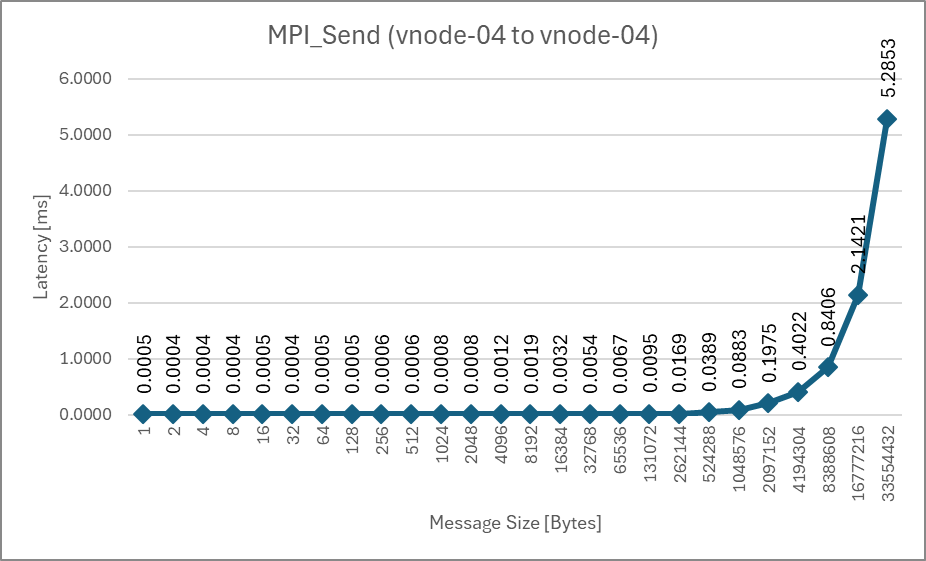
\includegraphics[width=0.49\textwidth]{images/part1/mpi-send-04-04-l.png}
\hfill
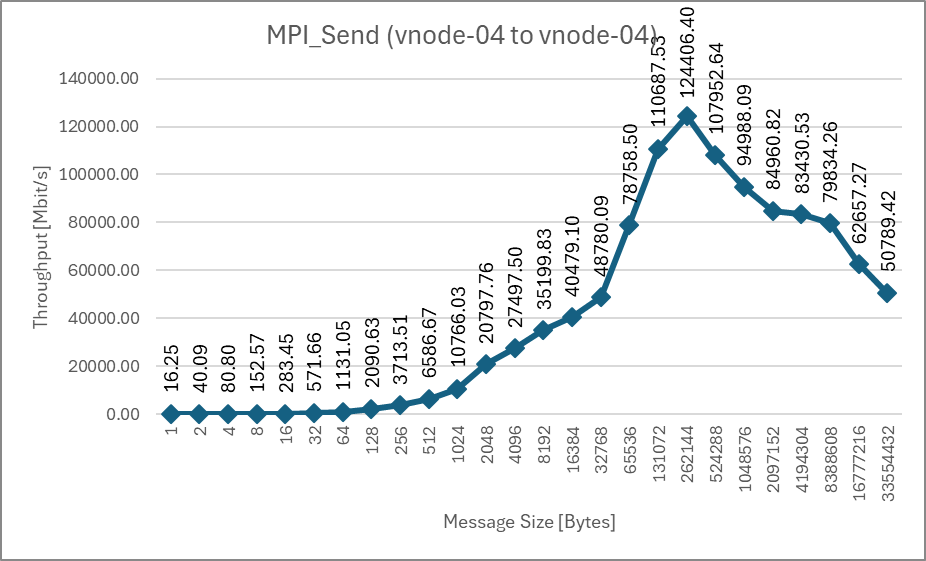
\includegraphics[width=0.49\textwidth]{images/part1/mpi-send-04-04-t.png}\\[0.5em]
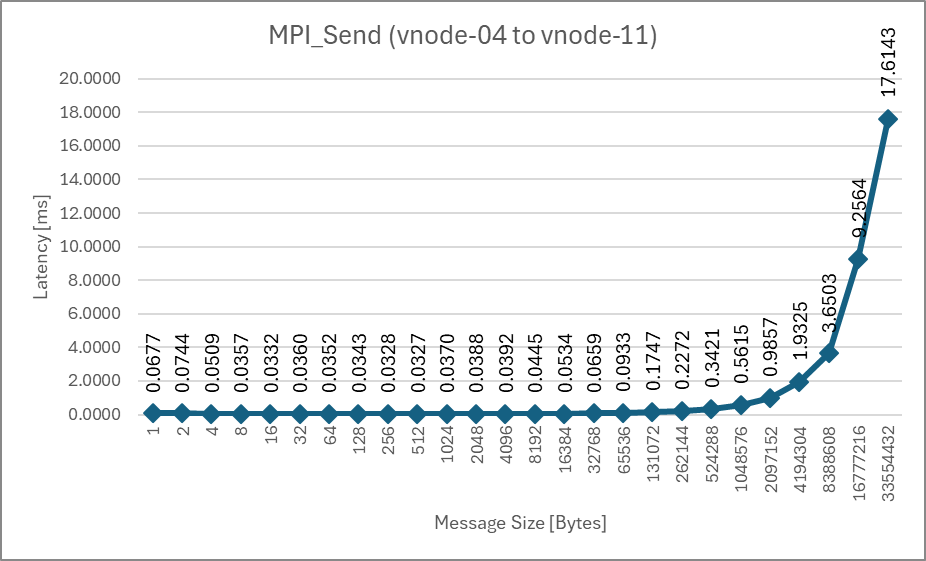
\includegraphics[width=0.49\textwidth]{images/part1/mpi-send-04-11-l.png}
\hfill
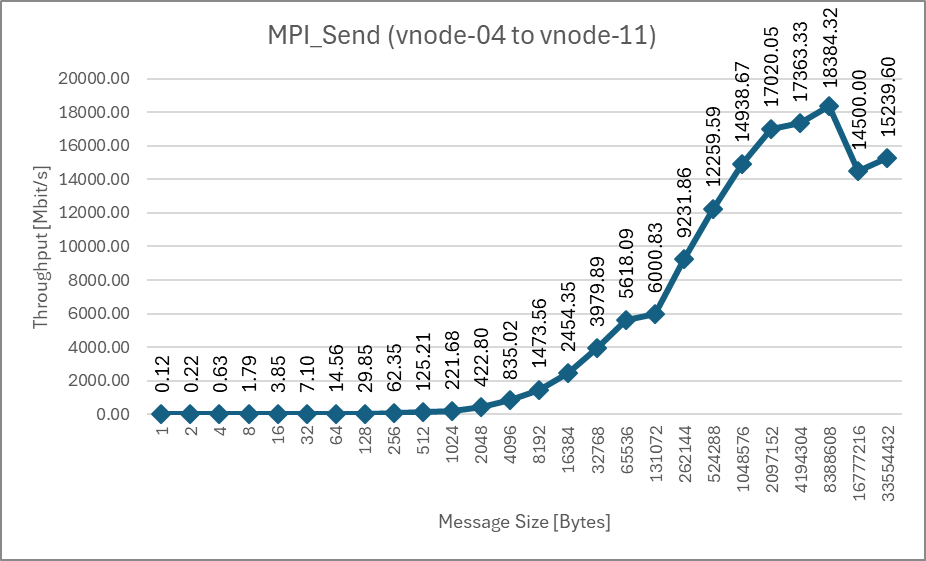
\includegraphics[width=0.49\textwidth]{images/part1/mpi-send-04-11-t.png}
\caption{Wyniki benchmarku dla \texttt{MPI\_Send} (układ 2x2).}
\label{fig:part1-mpi-send-grid}
\end{figure}

\begin{figure}[H]
\centering
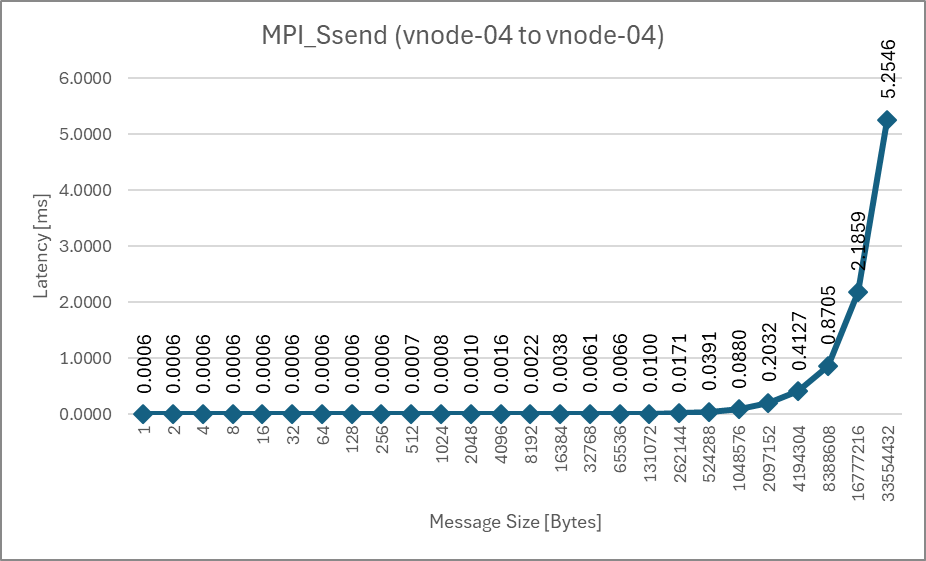
\includegraphics[width=0.49\textwidth]{images/part1/mpi-ssend-04-04-l.png}
\hfill
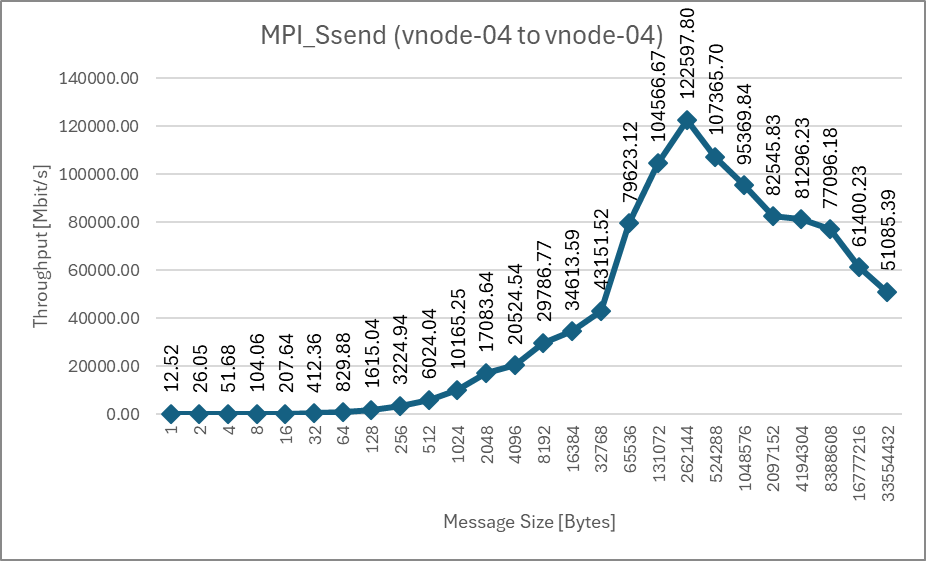
\includegraphics[width=0.49\textwidth]{images/part1/mpi-ssend-04-04-t.png}\\[0.5em]
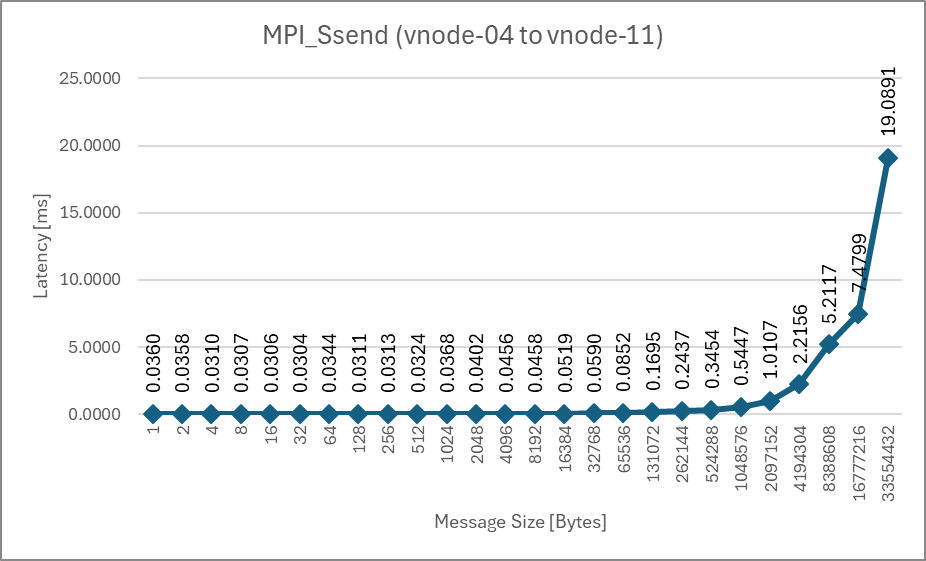
\includegraphics[width=0.49\textwidth]{images/part1/mpi-ssend-04-11-l.png}
\hfill
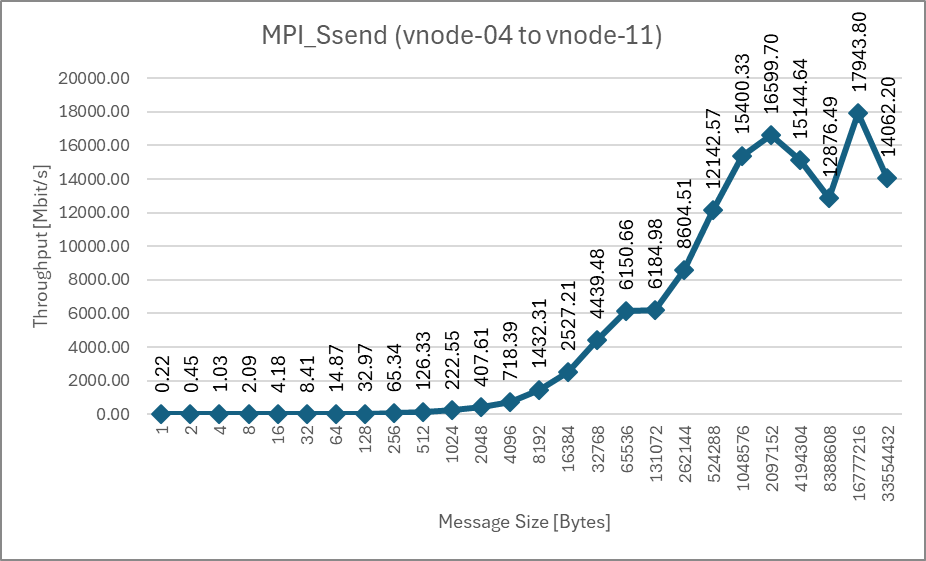
\includegraphics[width=0.49\textwidth]{images/part1/mpi-ssend-04-11-t.png}
\caption{Wyniki benchmarku dla \texttt{MPI\_Ssend} (układ 2x2).}
\label{fig:part1-mpi-ssend-grid}
\end{figure}

\section{Część 2: Przybliżanie liczby Pi metodą Monte Carlo}

\subsection{Opis algorytmu i implementacji}
Algorytm wykorzystuje stosunek pola koła do pola kwadratu: $\pi = 4 \cdot \frac{P_{c}}{P_{s}}$. 
Zrównoleglenie polega na podziale całkowitej liczby punktów do wylosowania pomiędzy procesy. 
Każdy proces liczy punkty wewnątrz okręgu, a wynik końcowy jest zbierany za pomocą operacji \texttt{MPI\_Reduce}.

Wykonano testy dla dwóch wariantów skalowania:
\begin{compactitem}
    \item \textbf{Prawo Amdahla (Skalowanie silne)}: liczba punktów jest stała, a liczba procesorów rośnie. W naszym przypadku wykorzystano równomierny podział pracy między procesory.
    \item \textbf{Prawo Gustafsona (Skalowanie słabe)}: liczba punktów rośnie proporcjonalnie do liczby procesorów. Tutaj każdy procesor otrzymuje stały rozmiar problemu, więc im więcej procesorów, tym większy jest całkowity rozmiar problemu.
\end{compactitem}

Prawo Amdahla mówi, że przyspieszenie jest ograniczone przez udział części sekwencyjnej, natomiast prawo Gustafsona zakłada, że część sekwencyjna pozostaje stała, natomiast zrównoleglona część rośnie wraz z liczbą procesorów. 
Przeanalizowano czasy wykonania w zależności od liczby procesorów, aby znaleźć przyspieszenie, efektywność oraz udział części sekwencyjnej dla obu wariantów skalowania. 

Spodziewaliśmy się, dobrego zrównoleglenia, z powodu, że losowanie metodą Monte Carlo jest problemem naturalnie równoległym, czyli takim w którym część niemożliwa do zrównoleglenia jest pomijalna i nie ma wpływu na czas wykonania. 
Nie skupiamy się na dokładności przybliżenia liczby $\pi$, dopóki jest ona w granicach rozsądku, ponieważ nie jest to główny cel tego zadania. 
Sprawdzono trzy rozmiary problemu: mały (najniższy mierzalny czas), średni i duży (czas wykonania około 1 minuty). Wykonano 10 pomiarów dla każdej konfiguracji, a wyniki uśredniono. 

Będziemy obserwować \textbf{przyspieszenie względne}, czyli odnoszące się do czasu wykonania na jednym procesorze algorytmu równoległego, a nie do czasu wykonania najlepszego algorytmu sekwencyjnego. 
Musimy mieć to na uwadzę, ponieważ może istnieć lepszy algorytm bazowy, który nie jest obarczony m.in. kosztem komunkacji.

Wprowadzimy oznaczenia przydatne przy dalszych metrykach:
\begin{compactitem}
    \item $n$ - liczba procesorów.
    \item $T_1$ - czas wykonania algorytmu na jednym procesorze.
    \item $T_n$ - czas wykonania algorytmu na $n$ procesorach.
\end{compactitem}
Co ważne wzory na poniższe metryki różnią się w zależności od tego, czy mówimy o prawie Amdahla, czy Gustafsona.

\subsection{Przyspieszenie}
Dla prawa Amdahla, przyspieszenie jest definiowane jako:
\[ S_n = \frac{T_1}{T(n)} \]
Dla prawa Gustafsona, przyspieszenie jest definiowane jako:
\[ S_n = n \cdot \frac{T_1}{T(n)} \]

Odchylenie standardowe, ze względu na propagację błedów, można obliczyć jako:
\[ \sigma_{S_n} = S_n \cdot \sqrt{ \left( \frac{\sigma_{T_1}}{\bar{T}_1} \right)^2 + \left( \frac{\sigma_{T_n}}{\bar{T}_n} \right)^2 } \]

Otrzymane wyniki przyspieszania przedstawiono na Rysunku \ref{fig:part2-speedup-1x2}. Są one w większości zgodne z oczekiwaniami, jednak istnieją pewne losowe odchylenia mogące wynikać z pracy komputera, na którym wykonywane były testy.

\begin{figure}[H]
\centering
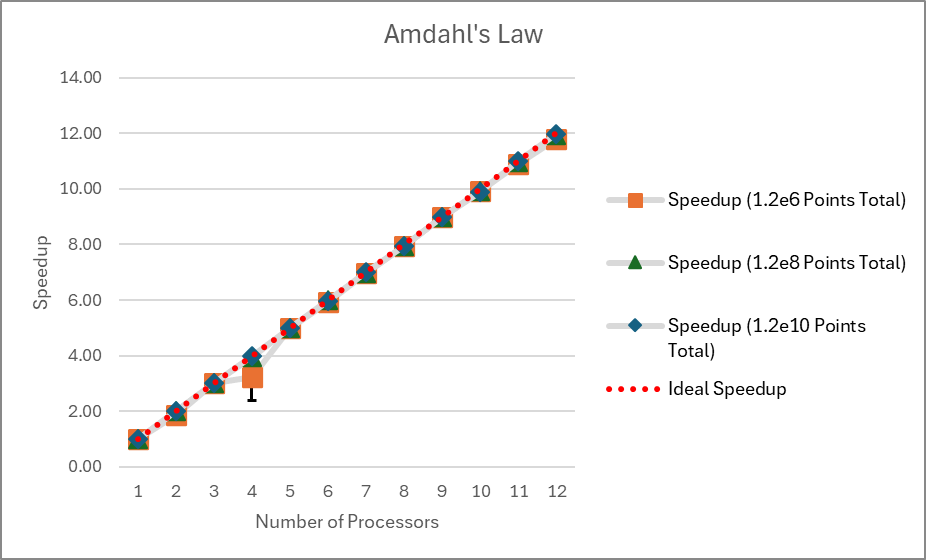
\includegraphics[width=0.49\textwidth]{images/part2/a-speedup.png}
\hfill
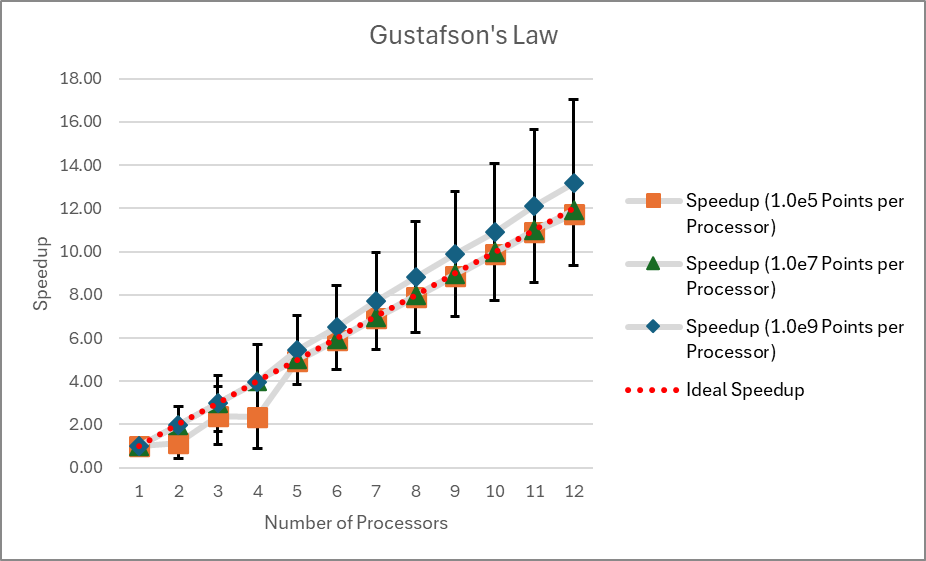
\includegraphics[width=0.49\textwidth]{images/part2/g-speedup.png}
\caption{Przyspieszenie (speedup): Amdahl (lewy wykres) i Gustafson (prawy wykres), układ 1x2.}
\label{fig:part2-speedup-1x2}
\end{figure}

\subsection{Efektywność}
Dla prawa Amdahla i Gustafsona efektywność jest definiowana jako:
\[ E_n = \frac{S_n}{n} \]
gdzie $S_n$ jest odpowiednio przyspieszeniem dla prawa Amdahla lub Gustafsona.

Odchylenie standardowe efektywności można obliczyć jako:
\[ \sigma_{E_n} = \frac{\sigma_{S_n}}{n} \]

Otrzymane wyniki efektywności przedstawiono na Rysunku \ref{fig:part2-efficiency-1x2}. Są widoczne losowe odchylenia podobnie jak w powyższym przypadku dla przyspieszenia.

\begin{figure}[H]
\centering
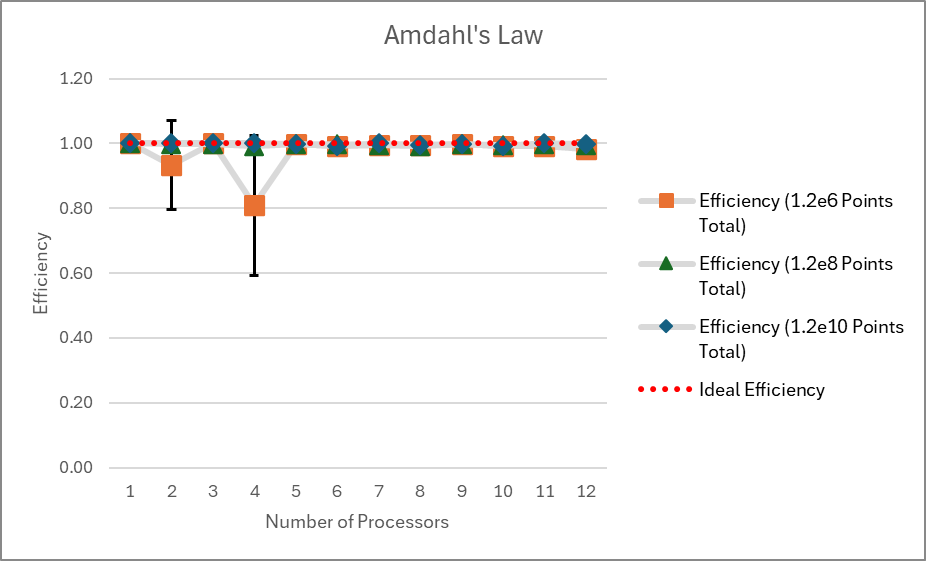
\includegraphics[width=0.49\textwidth]{images/part2/a-efficiency.png}
\hfill
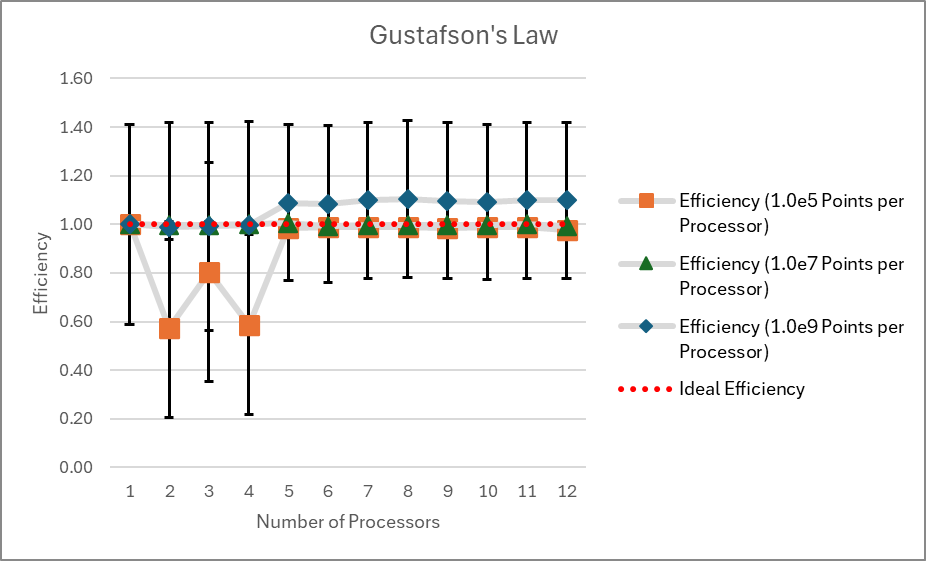
\includegraphics[width=0.49\textwidth]{images/part2/g-efficiency.png}
\caption{Efektywność (efficiency): Amdahl (lewy wykres) i Gustafson (prawy wykres), układ 1x2.}
\label{fig:part2-efficiency-1x2}
\end{figure}

\subsection{Udział części sekwencyjnej}
Dla prawa Amdahla, udział części sekwencyjnej jest definiowany jako:
\[ f = \frac{\frac{1}{S_n} - \frac{1}{n}}{1 - \frac{1}{n}} \]
Dla prawa Gustafsona, udział części sekwencyjnej jest definiowany jako:
\[ f = \frac{n - S_n}{n - 1} \]
gdzie $S_n$ jest odpowiednio przyspieszeniem dla prawa Amdahla lub Gustafsona.

Odchylenie standardowe udziału części sekwencyjnej można obliczyć jako:
\[ \sigma_{f} = \frac{\sigma_{S_n}}{n - 1} \]

Otrzymane wyniki udziału części sekwencyjnej przedstawiono na Rysunku \ref{fig:part2-serial-fraction-1x2}. Są one zgodne z oczekiwaniami, oraz także zawierają losowe odchylenia podobnie jak w powyższych przypadkach dla przyspieszenia i efektywności.

\begin{figure}[H]
\centering
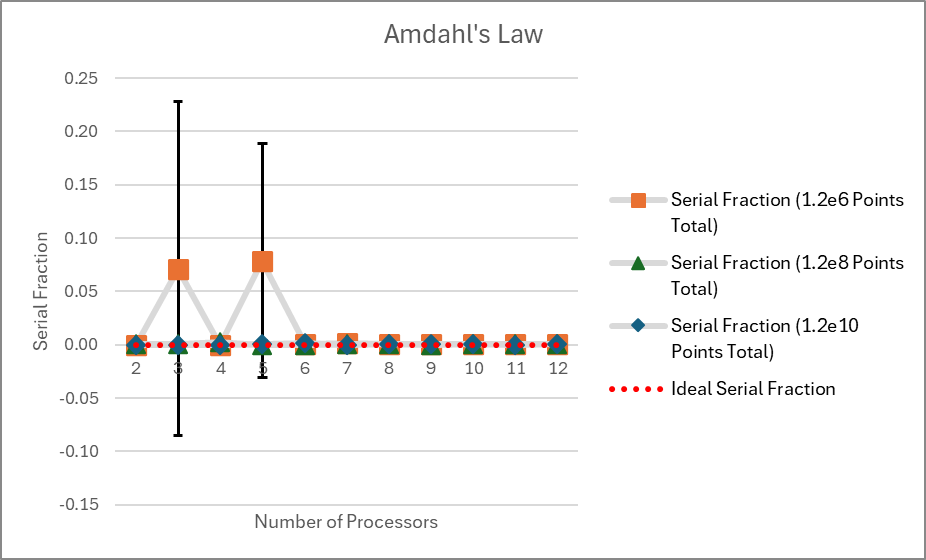
\includegraphics[width=0.49\textwidth]{images/part2/a-serial-fraction.png}
\hfill
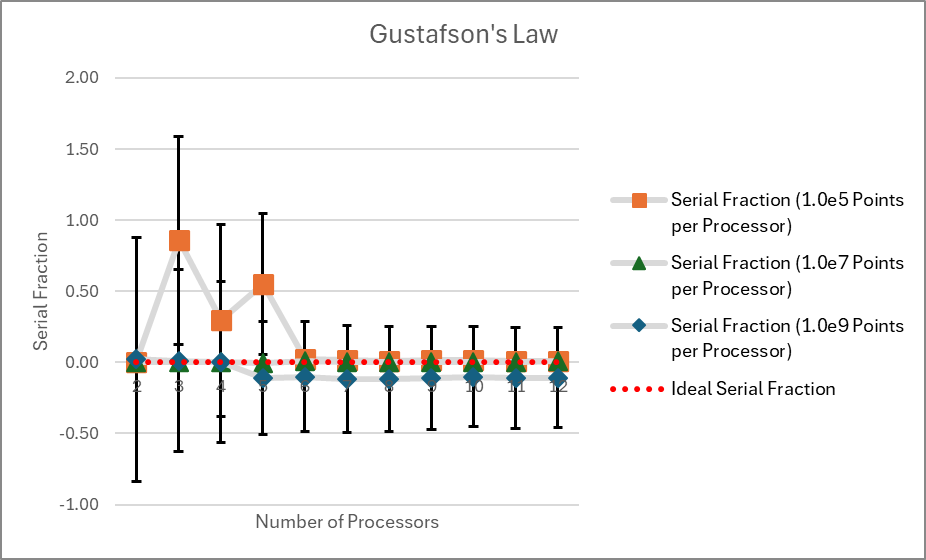
\includegraphics[width=0.49\textwidth]{images/part2/g-serial-fraction.png}
\caption{Udział części sekwencyjnej (serial fraction): Amdahl (lewy wykres) i Gustafson (prawy wykres), układ 1x2.}
\label{fig:part2-serial-fraction-1x2}
\end{figure}

\subsection{Czasy wykonania}

Przedstawione wyniki czasów wykonania (Rysunek \ref{fig:part2-time-vs-procs-grid}) pokazują, że czas wykonania maleje wraz ze wzrostem liczby procesorów, dla prawa Amdahla. 
Dla prawa Gustafsona, czas wykonania pozostaje mniej więcej stały, co jest zgodne z oczekiwaniami, ponieważ rozmiar problemu rośnie proporcjonalnie do liczby procesorów. 
Słupki błędów pokazują odchylenie standardowe, które mogą wskazywać na niestabilność pomiarów, co przełożyło się na wyniki metryk przyspieszenia, efektywności i udziału części sekwencyjnej.

\begin{figure}[H]
\centering
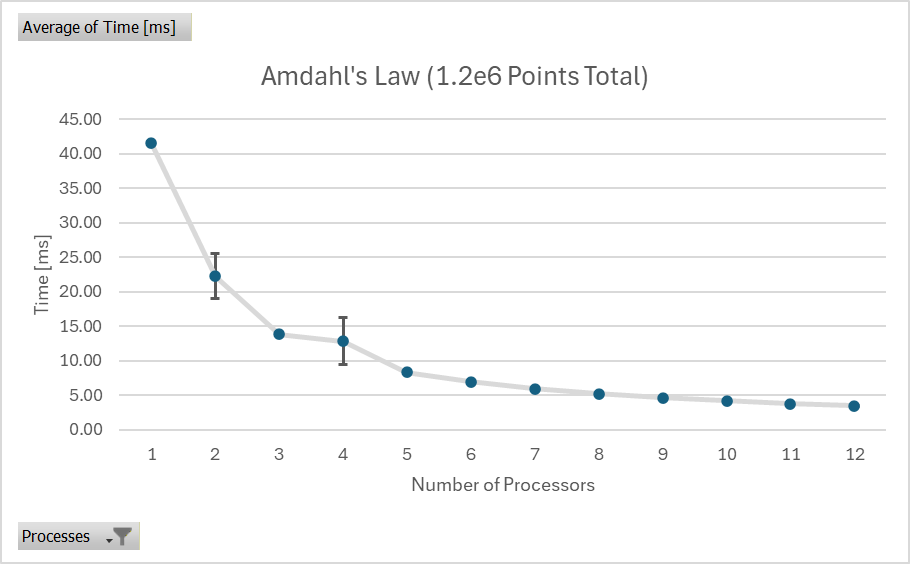
\includegraphics[width=0.49\textwidth]{images/part2/a-e6.png}
\hfill
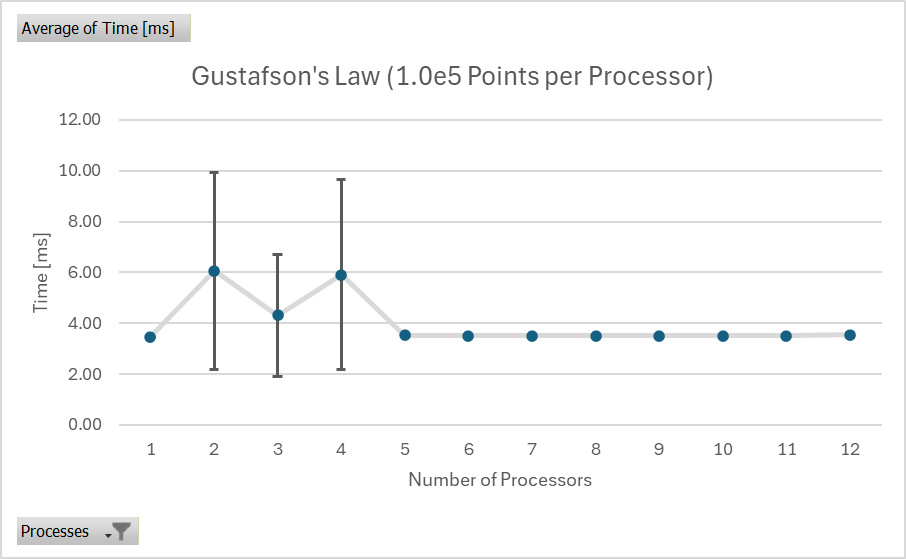
\includegraphics[width=0.49\textwidth]{images/part2/g-e5.png}\\[0.5em]
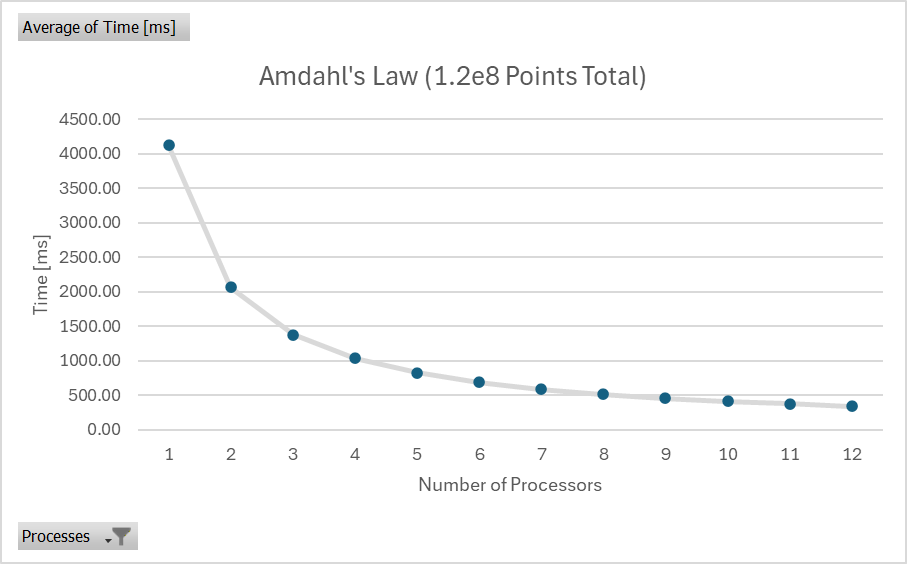
\includegraphics[width=0.49\textwidth]{images/part2/a-e8.png}
\hfill
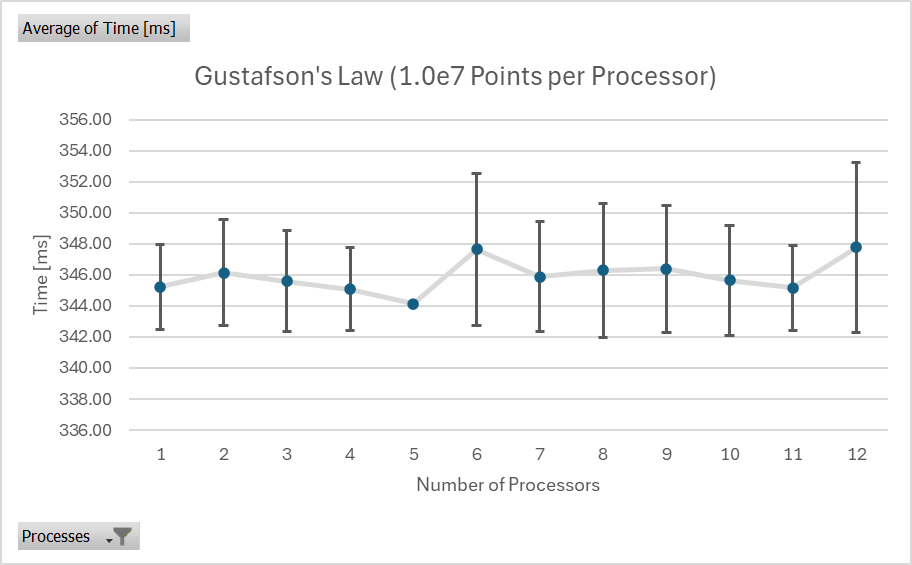
\includegraphics[width=0.49\textwidth]{images/part2/g-e7.png}\\[0.5em]
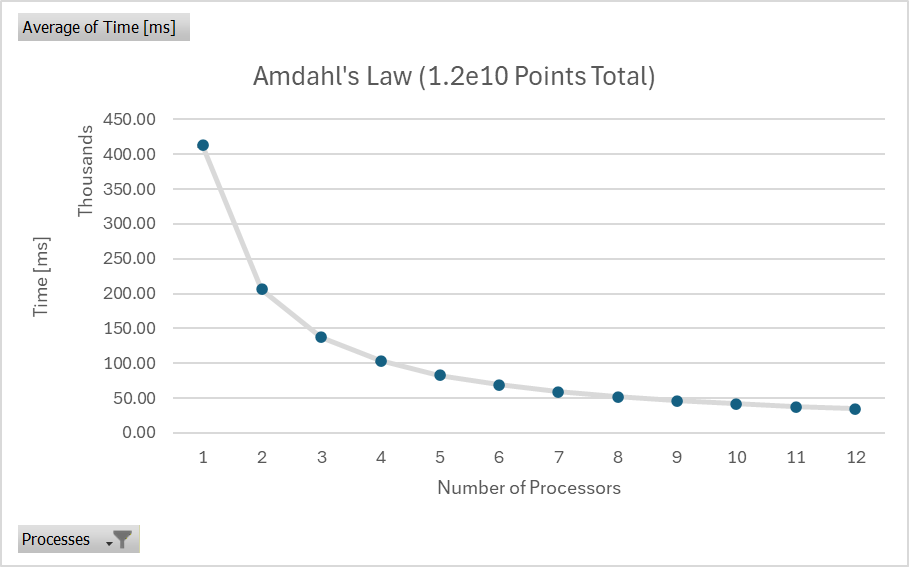
\includegraphics[width=0.49\textwidth]{images/part2/a-e10.png}
\hfill
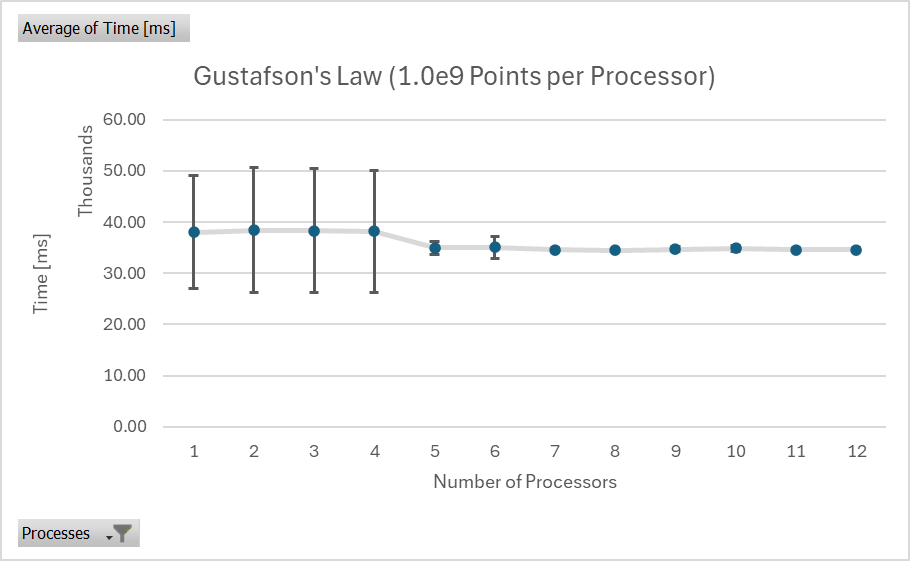
\includegraphics[width=0.49\textwidth]{images/part2/g-e9.png}
\caption{Czas wykonania w zależności od liczby procesorów (układ 3x2) dla konfiguracji Amdahla i Gustafsona.}
\label{fig:part2-time-vs-procs-grid}
\end{figure}

\subsection{Koszt komunikacji}
Narzut komunikacji jest nieznaczny, przy przesyłaniu danych typu \texttt{uint64\_t} w części 1. (rysunek \ref{fig:part1-mpi-send-grid}) koszt przesyłania komunikatów o rozmiarze 8B wynosił jedynie 0.0005 ms, co jest znacznie mniej niż czas wykonania algorytmu nawet dla małego rozmiaru problemu (5 ms). 
Mimo, że wykorzystujemy operację \texttt{MPI\_Reduce}, nie powinna ona znacząco wpłynąć na wyniki.


\newpage
\section{Podsumowanie}
Najważniejsze wnioski z przeprowadzonych testów to:
\begin{compactitem}
    \item Komunikacja wewnątrz węzła jest znacznie szybsza niż komunikacja między węzłami.
    \item Potrzebny jest dobór odpowiedniego rozmiaru komunikatów, aby osiągnąć optymalną przepustowość.
    \item Algorytm Monte Carlo do przybliżania liczby $\pi$ jest naturalnie równoległym, w którym część skewencyjna i narzut komunikacyjny są pomijalnie małe.
    \item Każde pomiary są obarczone pewnym błędęm, dlatego ważne jest wykonywanie wielu prób i analiza zgodności wyników z oczekiwaniami.
\end{compactitem}

\end{document}